%*----------- SLIDE -------------------------------------------------------------
\begin{frame}[t]{Metodologia}
    \begin{figure}
        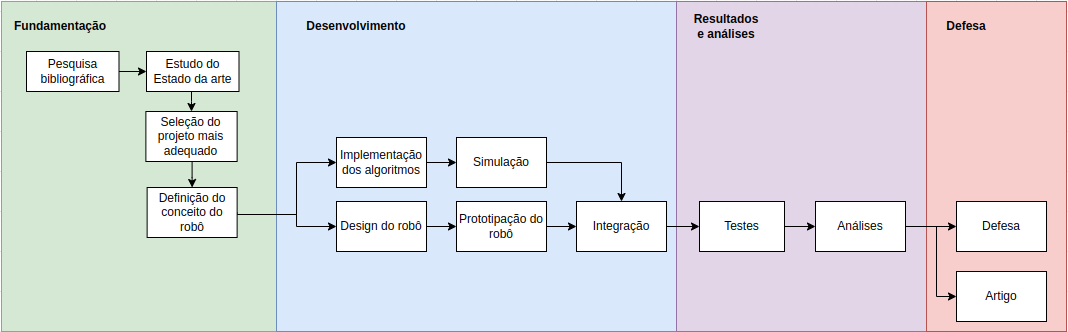
\includegraphics[width=1.0\textwidth]{metodologia.png}
        %\caption{.}
    \end{figure}
    %*----------- notes
    \note[item]{Notes can help you to remember important information. Turn on the notes option.}
\end{frame}
%-

%*----------- SLIDE -------------------------------------------------------------
\begin{frame}[t]{Fundamentação}
    Aplicamos o método Bili para buscar artigos de referência para o SOTA.

    O foco da pesquisa foi:
    \begin{itemize}
        \item Robô quadrúpede
        \item Design
        \item Estrutura
        \item Controle
    \end{itemize}


    %*----------- notes
    \note[item]{Notes can help you to remember important information. Turn on the notes option.}
\end{frame}
%-

%*----------- SLIDE -------------------------------------------------------------
\begin{frame}[t]{Fundamentação}
    \textbf{Requisitos do "cliente":}
    \begin{itemize}
        \item O robô deverá ser capaz de operar por tempo suficiente para inspecionar um ambiente semelhante a uma sala de aula
        \item O robô deverá ser capaz de se locomover em ambientes irregulares
        \item O robô deverá ser capaz de transpor obstáculos pequenos, similares a um livro
        \item O robô deverá atuar em ambientes indoor e outdoor
        \item O transporte do robô deve ser realizado por uma única pessoa utilizando uma maleta
        \item O robô deverá suportar um payload de 2 kg
    \end{itemize}

    %*----------- notes
    \note[item]{Notes can help you to remember important information. Turn on the notes option.}
\end{frame}
%-

%*----------- SLIDE -------------------------------------------------------------
\begin{frame}[t]{Fundamentação}
    \textbf{Requisitos técnicos:}
    \begin{itemize}
        \item O robô deverá possuir uma altura máxima de 500 mm
        \item O robô deverá possuir um comprimento máximo de 500 mm
        \item Deverá ter uma massa de, no máximo, 10 kg +/- 1
        \item As juntas devem ser atuadas por servomotores
        \item A relação de massa entre pernas/corpo deve ser a menor possível
        \item O robô deverá ser capaz de transpor obstáculos de até 5cm
        \item O robô deverá ser capaz de operar por, no mínimo, 20 minutos
    \end{itemize}

    %*----------- notes
    \note[item]{Notes can help you to remember important information. Turn on the notes option.}
\end{frame}
%-